%----------------------------------------------------------------------------------------
%	PACKAGES AND DOCUMENT CONFIGURATIONS
%----------------------------------------------------------------------------------------

\documentclass[12pt,a4paper]{article}

\usepackage[version=3]{mhchem} % Package for chemical equation typesetting
\usepackage{siunitx} % Provides the \SI{}{} and \si{} command for typesetting SI units
\usepackage{graphicx} % Required for the inclusion of images
\usepackage{natbib} % Required to change bibliography style to APA
\usepackage{amsmath} % Required for some math elements 
\usepackage{geometry}
\usepackage{enumerate}
\usepackage{float}
\usepackage{subfigure}
\usepackage{pdfpages}
\usepackage{siunitx}
\usepackage{fancyhdr}
\usepackage{textcomp}

\includepdfset{pagecommand={\thispagestyle{fancy}}}%page number for pdf

\renewcommand{\labelenumi}{\alph{enumi}.} % Make numbering in the enumerate environment by letter rather than number (e.g. section 6)
\geometry{left=2cm,right=2cm,top=3cm,bottom=3cm}

%\usepackage{times} % Uncomment to use the Times New Roman font

%----------------------------------------------------------------------------------------
%	DOCUMENT INFORMATION
%----------------------------------------------------------------------------------------


\begin{document}

\begin{center}
~\\
\rule[0mm]{400pt}{0.5pt}
\Large{ \textsc{\newline\\UM-SJTU Joint Institute\\Physics Laboratory\\(Vp141)\\}}
\rule[0mm]{400pt}{0.5pt}
\Large{ \textsc{\newline\newline\newline\newline\newline\newline\\
Laboratory Report\\}}
\Large{\textsc{ \\ Exercise 2  \\ Measurement of Fluid Viscosity} }

\end{center}

\begin{description}
    \item[] 
    \item[] 
    \item[] 
    \item[] 
    \item[] 
    \item[]
    \item[]\qquad \qquad Name: Han Yibei \qquad ID:519370910123   \qquad    Group:11\\
    \item[]\qquad \qquad Date: \today
\end{description}

\newpage

%----------------------------------------------------------------------------------------
%	SECTION 1
%----------------------------------------------------------------------------------------

\section{Introduction}

The objective of this experiment is to quantitatively express the fluid viscosity using the Stoke’s method. A moving object in a fluid receives a drag force which is related to both the physical property of the object and the property of the fluid. It also undergoes gravity and buoyancy force. By measuring some of the physical quantities and comparing these three forces we can express the viscosity coefficient $\eta$.

\section{Theoratical background}
\begin{itemize}
    \item A spherical object with radius R and speed v in an infinitely long cylindrical container with radius Rc receives a linear drag force, of which the direction is opposite to its velocity and the magnitude of it is:$$F_1=6\pi\eta vR(1+2.4\frac{R}{r_c})$$
    \item The magnitude of the upward buoyancy force it is acted upon is:$$F_2=\frac{4}{3}\pi R^3\rho_1g$$ where $\rho_1$ is the density of the fluid.
    \item The downward weight of the object can be expressed by$$F_3=\frac{4}{3}\pi R^3\rho_2g=mg$$ where m is the mass of the object.
    \item By substituting $\frac{s}{t}$ for v and solcing the relational expression $F_1+F_2=F_3$, we get the final expression of $$\eta=\frac{2}{9}gR^2\frac{(\rho_2-\rho_1)t}{s}\times\frac{1}{1+2.4\frac{R}{R_c}}=\frac{mg-\frac{4}{3}\pi R^3\rho_1g}{6\pi vR}\times \frac{1}{1+2.4\frac{R}{R_c}}$$
\end{itemize}
Besides, the length L may contribute to further corrections, which depends on the ratio
$R_c/L$.

\section{Apparatus}
The experimental setup is shown in figure 1.

\begin{figure}[h]
    \centering
    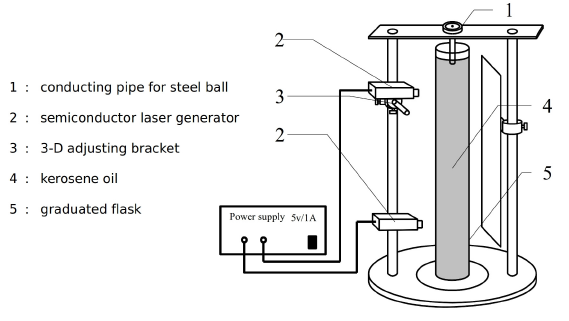
\includegraphics[width=10cm]{apparatus.png}
    \caption{Stoke's viscosity measurement apparatus}
\end{figure}

The experimental equipment is fixed on an iron support. A graduated flask is placed on the center with castor oil in it. The two semiconductor laser generators on the left are on the same vertical line. The laser they send out can travel through the fluid. The steel ball is dropped through the conducting pipe on the top.
For physical quantities measurement, a micrometer is used to measure the diameter of the steel ball. A caliper is used to measure the inner diameter of the graduated flask. A densimeter is used to measure the density of the castor oil. The mass of the steel ball is measured by an electronic scale. A ruler is used to measure the distance between the two laser beams. A stopwatch is used to measure the time cost by the ball travelling through the interval of the two laser beams. A thermometer placed in castor oil is used to measure the environment temperature.
The information of each measurement device is shown in Table 1.


\begin{table}[H]
    \centering
    \begin{tabular}{|c|c|c|c|}
        \hline
        Apparatus & Range & Minimum scale & Apparatus uncertainty\\
        \hline
        Micrometer & 25.00mm & 0.01mm & $\pm$0.005mm \\
        \hline
        Caliper & 125.00mm & 0.02mm & $\pm$0.02mm \\
        \hline
        Densimeter & 0.900-1.000$g/cm^3$ &  0.001$g/cm^3$ & $\pm$0.001$g/cm^3$ \\
        \hline
        Electronic scale & / & 0.001g & $\pm$ 0.001g \\
        \hline
        Ruler & 300mm & 1mm & $\pm$0.5mm \\
        \hline
        Stopwatch & / & 0.01s & $\pm$ 0.01s \\
        \hline
        Thermometer & -10-50.0\textcelsius & 0.5\textcelsius & $\pm$ 0.5\textcelsius\\
        \hline
    \end{tabular}
    \caption{Information of Each Measurement Device}
\end{table}
 
\section{Measurement}
The physical quantities we need for calculation are: \par
Environmental factors: temperature $T$, fluid density $ρ_1$, acceleration due to gravity $g$, \par
inner diameter of the graduated flask $D$
Ball properties: diameter of the ball $d$, the mass of one ball $m$ \par
Ball velocity $v$: the distance traveled $s$, time $t$ 

\subsection{Apparatus Adjustment}
\begin{enumerate}
    \item Adjust the knobs to make the plumb aiming at the center of the base.
    \item Turn on the two lasers, adjust the beams till they are parallel and aim at the plumb line.
    \item Remove the plumb and place the flask at the center of the base.
    \item Place the guiding pipe on the top of the device.
    \item Put a metal ball into the pipe and check whether the ball,  can blocks the laser beams. If not, repeat Step 1.
\end{enumerate}

\subsection{ Environmental factors measurement}
\begin{enumerate}
    \item Read and record the reading of the thermometer placed in castor oil.
    \item Read and record the reading of the densimeter.
    \item Use a caliper to measure the inner diameter of the graduated flask for 6 times. Record all the readings. 
\end{enumerate}

\subsection{Ball properties measurement}
\begin{enumerate}
    \item Use a micrometer to measure the diameter of one steel ball for 10 times. Record each reading. 
    \item To measure the mass of one ball, we choose to measure the total mass of 40 balls and then divide it by 40. In this step we have assumed that every ball is of the same size and mass. If the specifications of the balls are different, there will exist errors.
\end{enumerate}

\subsection{Ball velocity measurement} 
\begin{enumerate}
    \item The power supply is turned on, and the generator sets off two laser beams. Erect a ruler with its side facing the laser beams. Record the two readings where the two laser beams points at. Repeat this step for 3 times. In this step, we record the two readings and then subtract them to get the distance the ball travels. 
    \item One ball is dropped from the conducting pipe each time. The timer is started as soon as the ball passes the first laser beam and is stopped when the ball passes the second beam.
    \item Repeat step b until 6 sets of valid time are recorded.
\end{enumerate}
In step 2, there existing two spot on the ruler means that the two laser generators are at the same vertical line. Since the ball has a small possibility to follow a route that exactly intersects with the range of the laser beam, step 3 must be repeated several times to achieve 6 valid time lengths. What’s more, error exists in this step because the time is recorded by human who has reaction time. There might be inaccuracy in measuring the time.

\section{Result}
\subsection{Environmental Factors Measurement}
Fluid Density: $\rho_1=0.956\pm 0.001g/cm^3=956\pm 1kg/m^3$\par 
Temperature: $T=23\pm 0.5$\textcelsius \par 
Acceleration due to gravity (given by instructor): $g=9.794m/s^2$
\begin{table}[H]
    \centering
    \begin{tabular}{|c|c|}
        \hline
        \multicolumn{2}{|c|}{diameter D [mm]$\pm$0.02mm} \\
        \hline
        D1 & 60.29 \\
        \hline  
        D2 & 60.08 \\
        \hline 
        D3 & 60.34 \\
        \hline
        D4 & 60.20 \\
        \hline 
        D5 & 60.22 \\
        \hline
        D6 & 60.36 \\
        \hline
    \end{tabular}
    \caption{ Measurement data for the inner diameter of the flask}
\end{table}
From table 2 we get the average inner diameter of the flask is:
$$\begin{aligned}
    \overline{D}=\frac{1}{6}\sum^6_{n=1}D_n=&\frac{60.29+60.08+60.34+60.20+60.22+60.36}{6}=60.25\pm0.11mm\\
    &=0.06025\pm0.00011m
\end{aligned}$$

\subsection{Ball Density Measurement}
\subsubsection{The diameter of the ball}
\begin{table}[H]
    \centering
    \begin{tabular}{|c|c||c|c|}
        \hline
        \multicolumn{4}{|c|}{diameter D [mm]$\pm$0.01mm} \\
        \hline
        d1 & 2.000 & d6 & 2.001 \\
        \hline 
        d2 & 1.998 & d7 & 1.998 \\
        \hline
        d3 & 1.997 & d8 & 1.999 \\
        \hline 
        d4 & 1.999 & d9 & 1.995 \\
        \hline
        d5 & 2.003 & d10 & 1.996 \\
        \hline
    \end{tabular}
    \caption{Measurement data for the diameter of the balls}
\end{table}
From table 3 we get the average diameter of the ball is: $\overline{d}=\frac{1}{10}\sum_{n=1}^{10}d_n=1.999\pm 0.005mm=0.00199\pm 0.00005m$.

\subsubsection{The mass of one ball}
Mass of 40 metal balls $M=1.312\pm0.001g=(1.312\pm 0.001)\times 10^-3kg$.\par
Consider the uncertainty, the mass of one ball $m=\frac{1.312}{40}=0.03280\pm 0.00003g=0.00003280 \pm 0.00000003kg$.

\subsection{Basll Velocity Measurement}
\subsubsection{The distance traveled}

\begin{table}[h]
    \centering
    \begin{tabular}{|c|c|c|c|c|c|}
        \hline
        \multicolumn{6}{|c|}{distance x[mm]$\pm$1[mm]} \\
        \hline
        xA,1 & 10.0 & xB,1 & 183.3 & S1 & 173.3 \\
        \hline
        xA,2 & 30.0 & xB,2 & 203.2 & S2 & 173.2 \\
        \hline
        xA,3 & 50.0 & xB,3 & 223.4 & S3 & 173.4 \\
        \hline
    \end{tabular}
    \caption{Distance measurement data}
\end{table}
The data in the last column are the results of the data in the second column subtracting from the data in the fourth column.
From the table we can get the average distance the ball travels is:
$$\overline{S}=\frac{1}{3}\sum^3_{n=1}S_n=\frac{173.3+173.2+173.4}{3}mm=173.3mm=0.1733mm$$
Consider the uncertainty, we get $S= 173.3\pm0.7mm=0.1733\pm0.0007m$

\subsubsection{The time cost}
\begin{table}[h]
    \centering
    \begin{tabular}{|c|c|}
        \hline
        \multicolumn{2}{|c|}{time t [s]$\pm$0.01s} \\
        \hline
        t1 & 8.63 \\
        \hline  
        t2 & 8.75 \\
        \hline 
        t3 & 8.58 \\
        \hline
        t4 & 8.68 \\
        \hline 
        t5 & 8.64 \\
        \hline
        t6 & 8.59 \\
        \hline
    \end{tabular}
    \caption{Time Measurement data}
\end{table}
From table 5 we can get the average time the ball travel is: 
$$\overline{t}=\frac{1}{6}\sum^6_{n=1}t_n=\frac{8.63+8.75+8.58+8.68+8.64+8.59}{6}s=8.65s$$
Consider the uncertainty, we get $t=8.65\pm 0.07s$

\subsubsection{The velocity of the ball}
Use equation $v=\frac{S}{t}$, we get$\overline{v}=\frac{\overline{S}}{t}=\frac{173.3}{8.645}mm/s=20.05mm/s$\par 
Consider the uncertainty, we get
$v=20.05\pm0.18 mm/s=0.02005\pm 0.00018m/s$

\subsection{Calculation of the fluid viscosity}
According to Eq.1
$$\eta=\frac{mg-\frac{4}{3}\pi R^3 \rho_1 g}{6\pi vR}\times\frac{1}{1+2.4\frac{R}{R_c}}=\frac{mg-\frac{4}{3}\pi (\frac{d}{2})^3 \rho_1 g}{6\pi v\frac{d}{2}}\times\frac{1}{1+2.4\frac{d}{D}}$$
$$=\frac{0.0000328kg\times 9.794m/s^2-\frac{4}{3}\times\pi\times (\frac{0.00199}{2}m)^3\times 956kg/m^3\times 9.794m/s^2}{6\times\pi\times 0.02005m/s\times \frac{0.00199}{2}m}\times\frac{1}{1+2.4\frac{0.00199m}{0.06025m}}$$
$$=0.70kg/ms$$
Consider the uncertainty, we get the viscosity of the fluid is $\eta=0.70\pm0.03 kg/m∙s$ \par
The relative difference is $\frac{|\eta-\eta_{theo}|}{\eta_{theo}}\times 100\%=\frac{|0.70-0.65|}{0.65}\times 100\%=7.7\%$


\section{Concludsion and Discussion}
In this experiment, we apply the knowledge of stoke’s method and measured the viscosity of castor oil at $t=23\pm 0.5$\textcelsius, which is $\eta =0.70\pm kg/m∙s$.
According to authoritative data, the viscosity of castor oil at T=300K is 0.650 kg/m∙s [1], which indicates that our experimental data is larger than standard. Below is the error analysis.
\begin{itemize}
    \item As our experimental data is relative larger, considering equation (1) we assume the radius of the ball might be measured smaller than reality. This error might result from the misuse of the micrometer. For example, the ball might not be put onto the anvil entirely so that the reading was smaller than its diameter. The density of the ball calculated using the experimental data is approximately 20$g/cm^3$, which is too big and proves the possibility of this error.
    \item Error might also exist if the ball had not reached the constant velocity. Since the flask is not long enough, the actual constant velocity might be larger than the measured velocity. This will result in a larger $\eta$.
    \item Since the stopwatch is started and stopped by human, there might exist error in time measuring. 
    \item The refraction effect of the light in the oil might cause errors, too.
\end{itemize} \par

To make the result more accurate, some improvements can be made:
\begin{itemize}
    \item Let machines detect the ball velocity. For example, a photoelectric gate sensor can be used. It will also eliminate the error caused by the velocity not reaching a constant value if the velocity is detected at different positions.
    \item Release the balls in the fluid to eliminate the possibility that bubbles stick to the surface of the balls.
\end{itemize}

\section{Reference}
\qquad [1] Standard viscosity of the castor oil: $https://www.engineeringtoolbox.com/absolute-viscosity-liquids-d\underline{~~}1259.html$\par
[2] Jiang Shaopeng, Qin Tian, Feng Yaming, Mateusz Krzyzosiak, Exercise 2 Measurement of Fluid Viscosity
	
	


\newpage
{\LARGE\textbf{APPENDIX}}
\setcounter{section}{0}
\renewcommand\thesection{\Alph{section}}

\section{Measurement Uncertainty Analysis}
\subsection{Uncertainty of Environmental factors}

\subsubsection{Uncertainty of the fluid density}
The maximum error of the densimeter is $1\times 10^{-3}g/cm^3$; therefore, $u_{\rho_1}=1\times 10^{-3} g/cm^3$.

\subsubsection{Uncertainty of the Temperature}
The maximum error of the thermometer is $0.5$\textcelsius; therefore, $u_T=0.5$\textcelsius

\subsubsection{Uncertainty of the Inner Diameter of the Flask}
$$\overline{D}=60.58mm$$
As the maximum uncertainty of the caliper is 0.02mm,$\Delta_B=0.02mm$. n=6, so $$\Delta_A=\frac{t_{0.95}}{\sqrt{n}}S_D=\frac{t_{0.95}}{\sqrt{n}}\sqrt{\frac{1}{n-1}\sum^n_{i=1}(D_i-\overline{D})^2}=0.11mm$$ \par 
The total uncertainty$u_D=\sqrt{{\Delta_A}^2+{\Delta_B}^2}=0.11mm$\par 
The corresponding relative uncertainty $u_{rD}=\frac{u_D}{\overline{D}}\times 100\%=0.18\%$ \par 
Therefore, the experimental found inner diameter of the flask $D=60.58\pm 0.11mm$

\subsection{Uncertainty about Ball properties}

\subsubsection{Uncertainty of the Diameter of the ball}
$$\overline{d}=1.999mm$$
As the maximum uncertainty of the micrometer is 0.005mm, $\Delta_B=0.005mm$. \par 
n=10, so $\Delta_A=\frac{t_{0.95}}{\sqrt{n}}S_d=\frac{t_{0.95}}{\sqrt{n}}\sqrt{\frac{1}{n-1}\sum^n_{i=1}(d_i-\overline{d})^2}=0.0017mm$
$$u_D=\sqrt{{\Delta_A}^2+{\Delta_B}^2}=0.005mm$$ \par
The total uncertainty $u_d=\sqrt{{\Delta_A}^2+{\Delta_B}^2}=0.005mm$\par 
The corresponding relative uncertainty $u_{rd}=\frac{u_d}{\overline{d}}\times 100\%=0.25\%$ \par 
Therefore, the experimental found diameter of the ball $D=1.999 \pm 0.005mm$

\subsubsection{Uncertainty of the Mass of one ball}
As the minimum scale of value of the electronic scale is 0.001g, $u_{m40}=0.001g$.Since $m=\frac{m40}{40}$, $\frac{\partial_{m40}}{\partial_m}=\frac{1}{40}$, so $u_m=\frac{1}{40}u_{m40}=\frac{1}{40}\times 0.001g=0.00003g$

\subsection{Uncertainty of the Ball Velocity}
\subsubsection{Uncertainty of the Distance the Ball Travel}
The uncertainty of xA and xB, the maximum uncertainty of the $\Delta_{xA,B}=0.5mm$, $\Delta_{xB,B}=0.5mm$. Since $S=xB-xA$, $\Delta_{S,B}=\sqrt{{\Delta_{xA,B}}^2+{\Delta_{xB,B}}^2}=0.7mm$ \par 
$$\overline{S}=173.3mm$$
n=3, so $$\Delta_A=\frac{t_{0.95}}{\sqrt{n}}S_S=\frac{t_{0.95}}{\sqrt{n}}\sqrt{\frac{1}{n-1}\sum^n_{i=1}(S_i-\overline{S})^2}=0.2mm$$
$$u_S=\sqrt{{\Delta_A}^2+{\Delta_B}^2}=0.7mm$$ \par
The total uncertainty $u_t=\sqrt{{\Delta_A}^2+{\Delta_B}^2}=0.07s$\par 
The corresponding relative uncertainty $u_{rt}=\frac{u_t}{\overline{t}}\times 100\%=0.81\%$ \par 
Therefore, the experimental found diameter of the ball $D=173.3\pm 0.7mm$


\subsubsection{Uncertainty of the Time Cost}
$$\overline{t}=8.65s$$
As the maximum uncertainty of the stopwatch is 0.01s, $\Delta_B=0.01s$. \par 
n=6, so $$\Delta_A=\frac{t_{0.95}}{\sqrt{n}}S_t=\frac{t_{0.95}}{\sqrt{n}}\sqrt{\frac{1}{n-1}\sum^n_{i=1}(t_i-\overline{t})^2}=0.07s$$
$$u_t=\sqrt{{\Delta_A}^2+{\Delta_B}^2}=0.07s$$ \par
The total uncertainty $u_S=\sqrt{{\Delta_A}^2+{\Delta_B}^2}=0.7mm$\par 
The corresponding relative uncertainty $u_{rS}=\frac{u_S}{\overline{S}}\times 100\%=0.40\%$ \par 
Therefore, the experimental found diameter of the ball $D=8.65 \pm 0.07s$

\subsubsection{Uncertainty of the Velocity}
$$v=\frac{S}{t}$$
$$\frac{\partial v}{\partial_S}=\frac{1}{t}$$
$$\frac{\partial v}{\partial_t}=-\frac{s}{t^2}$$
$$u_v=\sqrt{(\frac{\partial_v}{\partial_S})^2{u_s}^2+(\frac{\partial_v}{\partial_t})^2{u_t}^2}=\sqrt{(\frac{1}{8.65})^2\times 0.7^2+(-\frac{173.3}{8.65^2})^2\times 0.05^2}=0.18mm/s$$
The corresponding relative uncertainty $$u_{rv}=\frac{u_v}{\overline{v}}\times 100\%=0.90\%$$\par
Therefore, the experimental found velocity of the ball $D=20.05 \pm 0.18mm/s$

\subsection{Uncertainty of the Fluid Viscosity}
$$\eta=\frac{mg-\frac{4}{3}\pi(\frac{d}{2})^3\rho_1g}{6\pi v (\frac{d}{2})}\frac{1}{1+2.4\frac{d}{D}}$$
$$\frac{\partial_\eta}{\partial_m}=\frac{g}{3\pi vd}\frac{1}{1+2.4\frac{d}{D}}$$
$$\frac{\partial_\eta}{\partial_d}=(\frac{2d^2\rho_1g}{15vD}-\frac{4mg}{5\pi vdD})\frac{1}{(1+2.4\frac{d}{D})^2}-(\frac{mg}{3\pi vd^2}+\frac{\rho_1gd}{9v})\frac{1}{1+2.4\frac{d}{D}}$$
$$\frac{\partial_\eta}{\partial_{\rho_1}}=-\frac{d^2g}{18v}\frac{1}{1+2.4\frac{d}{D}}$$
$$\frac{\partial_\eta}{\partial_v}=\frac{\frac{1}{6}\pi d^3\rho_1g-mg}{3\pi d}\frac{1}{1+2.4\frac{d}{D}}\frac{1}{v^2}$$
$$\frac{\partial_\eta}{\partial_D}=\frac{12mg-2\pi d^3\rho_1g}{15\pi v}(\frac{1}{D+2.4d})^2$$
$$u_\eta=\sqrt{(\frac{\partial_\eta}{\partial_m})^2{u_m}^2+(\frac{\partial_\eta}{\partial_d})^2{u_d}^2+(\frac{\partial_\eta}{\partial_{\rho_1}})^2{u_{\rho_1}}^2+(\frac{\partial_\eta}{\partial_v})^2{u_v}^2}+(\frac{\partial_\eta}{\partial_D}{u_D}^2)=0.03kg/m\cdot s$$
$u_{r\eta}=\frac{u_\eta}{\eta}\times 100\%=4.29\%$

\section{Data Sheet}

\end{document}